\chapter{Problem Life Cycle}

\section{Problems Identification:} This research underscores the imperative to bolster data security and privacy in the dynamic
landscape of cloud storage. By delving into diverse encryption methodologies such as one-to-many
encryption, data integrity, resilient data deletion, and privacy-preserving solutions, the study
employs advanced technologies like identity-based encryption (IBE), attribute-based encryption
(ABE), homomorphic encryption, and searchable encryption. A noteworthy innovation lies in
strategically integrating a load balancer with GitHub, optimizing resource utilization and ensuring a
balanced distribution of data by creating multiple repositories for a single user. This approach
addresses potential vulnerabilities and contributes to efficient data management. Additionally, the
research explores post-quantum encryption to counter emerging threats, shedding light on
encryption principles and potential new models. Emphasizing the ongoing necessity for exploration
in data encryption technologies, the study positions itself as a commitment to advancing the field,
with future research planned to precisely align encryption methods with evolving security
requirements, ensuring robust and resilient data protection in cloud storage environments. 


\section{Problem Selection: } The research addresses the critical challenge of enhancing data security and privacy in cloud storage,
recognizing the evolving nature of security threats. The specific problem identified is the need for
effective encryption methodologies to safeguard user data, encompassing aspects such as one-tomany encryption, data integrity, resilient data deletion, and privacy-preserving solutions. The research
also acknowledges the emerging threats in the post-quantum era, emphasizing the imperative to
explore advanced encryption models to fortify cloud storage security against evolving risks

\section{Problem Definition: } The research focuses on the challenge of fortifying data security and privacy in cloud storage. The
problem is defined by the necessity for robust encryption methodologies, including one-to-many
encryption, data integrity assurance, resilient data deletion mechanisms, and privacy-preserving
solutions. The study also addresses the emerging threats in the post-quantum era, necessitating
exploration into advanced encryption models. The problem statement emphasizes the need for
effective measures to secure user data in the dynamically evolving landscape of cloud storage,
acknowledging the complexity of modern security risks. 

\section {Problem Analysis: } The analysis of the identified problem reveals a gap in current data security measures within cloud
storage. Existing encryption methodologies are scrutinized for their limitations in addressing oneto-many encryption, data integrity assurance, and resilient data deletion. The potential
vulnerabilities in privacy protection highlight the necessity for innovative solutions. Moreover, the
examination of emerging threats in the post-quantum era underscores the urgency of adapting
advanced encryption models. This problem analysis sets the stage for the research's exploration and
development of more effective security measures. 


\section {Fish Bone Diagram: } 
\begin{figure}[h]
  \centering
  \fbox{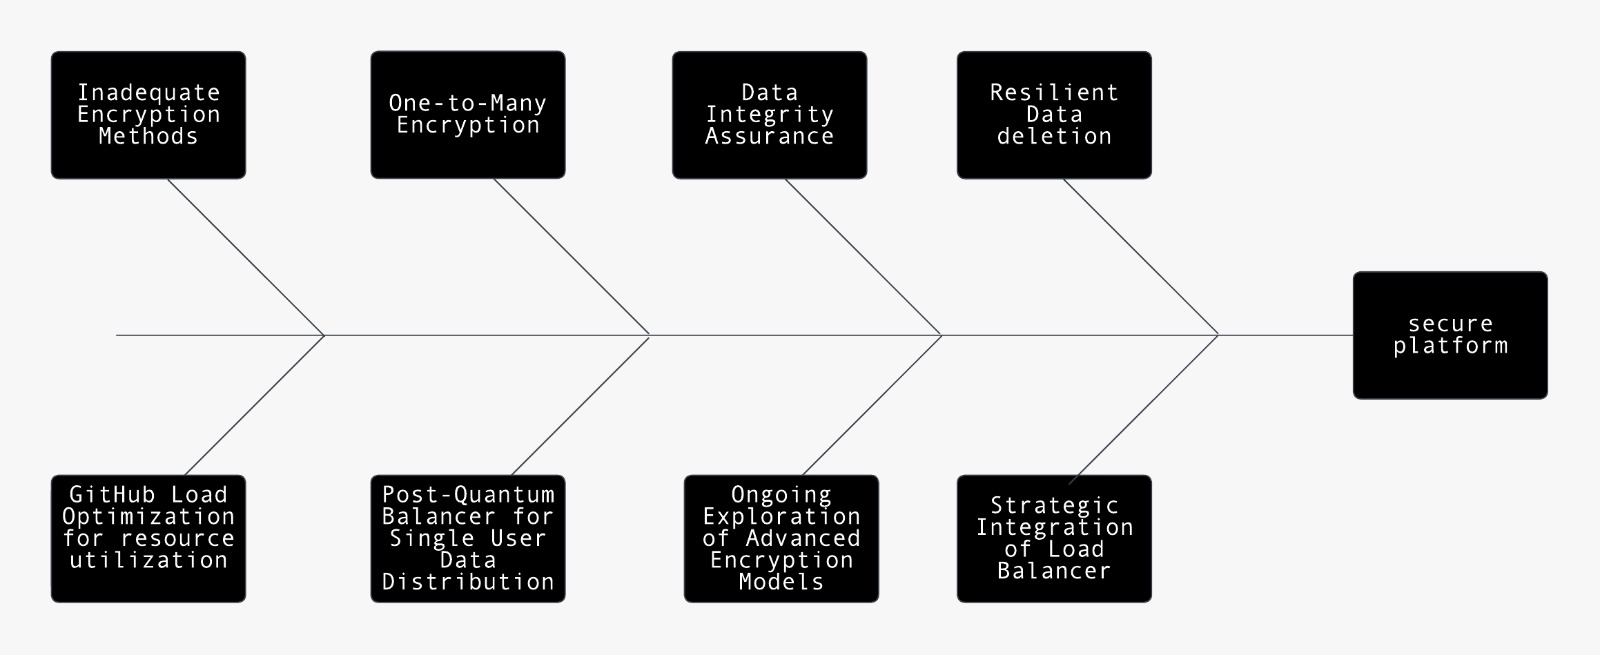
\includegraphics[height=85mm,width=85mm]{Images_Cloud/fishborn_diagram.png}}
  \caption{Fish Bone Diagram}
  
\end{figure}


\section {End Users:} End users who would benefit from the findings of this problem identification include individuals
and organizations utilizing cloud storage services.\\
\\
\textbf{Individual Users}: Everyday users who store personal data, documents, or sensitive information in
cloud storage platforms would directly benefit from enhanced data security and privacy measures.
The incorporation of advanced encryption methodologies ensures that their personal data remains
secure, and the strategic use of a load balancer with GitHub provides them with an optimized and
efficient data management experience
\\
\\
\textbf{Businesses and Enterprises}: Companies relying on cloud storage for their operations and data
management would find value in the research findings. The proposed encryption solutions,
including one-to-many encryption and resilience against data deletion, contribute to safeguarding
critical business information. The load balancing approach can also be particularly beneficial for
organizations with complex data distribution needs.
\\
\\
\textbf{Cloud Service Providers}: Entities offering cloud storage services stand to gain insights into
potential gaps in their current security measures. The research offers a roadmap for enhancing
encryption methodologies, which could be implemented by service providers to strengthen their
overall security infrastructure. This, in turn, would enhance their credibility and attract more users
concerned about data security.
\\
\\
\textbf{IT Security Professionals}: Security professionals responsible for maintaining and improving the
security posture of cloud storage systems would find the research beneficial. The analysis of current encryption methodologies and the identification of potential vulnerabilities provide valuable
information for security professionals to address weaknesses and proactively enhance security
protocols. 
\\
\\
\textbf{Researchers and Academia}: Scholars and researchers in the fields of cybersecurity, cloud
computing, and data protection would find this research useful for understanding current challenges
and proposing innovative solutions. It provides a foundation for further academic exploration and
development of advanced encryption models in the context of cloud storage.
In summary, the end users encompass a broad spectrum, ranging from individual users seeking
personal data protection to businesses, cloud service providers, IT security professionals, and
researchers aiming to advance the field of data security in cloud storage. The research findings offer
practical insights and solutions that can be applied to enhance the security and privacy of data in
cloud storage environments. 


\clearpage

